\section{Aspects of Development}

In this section, we will explain and discuss the solutions we used to implement
a Pentago game over \textit{MATLAB}.  Firstly, we dedicate a section to detail
the main aspects concerning the graphical interface and its components. In this
small section, we describe the general structure of the game, including the
approach we have chosen to organize the progress of the program. Then, the next
sections are dedicated to the heart of our program, which is the algorithm used
to simulate an artificial intelligence.

\vspace{10pt}

It is important to say that only the most important parts of the program are
fully explained. In order to visualize all code, please refer to the files
which will be indicated in the next sections.

\subsection{Graphical Interface - GUI}

All the code used in this item can be found in file \textbf{pentago\_plateau.m}

\vspace{10pt}

The window which can be seen in Figure \ref{fig:gui} shows the graphical
interface of the Pentago game. It is composed by two buttons  (\textit{‘Start
Game’} and \textit{‘Reset Game’}), a textbox (initially with ‘\textit{Press
[Start Game] to start.}’), whose function is to inform the player about the
current state of the game,  and a 6x6-slot matrix, which represents the board.

\begin{figure}[h]
\centering
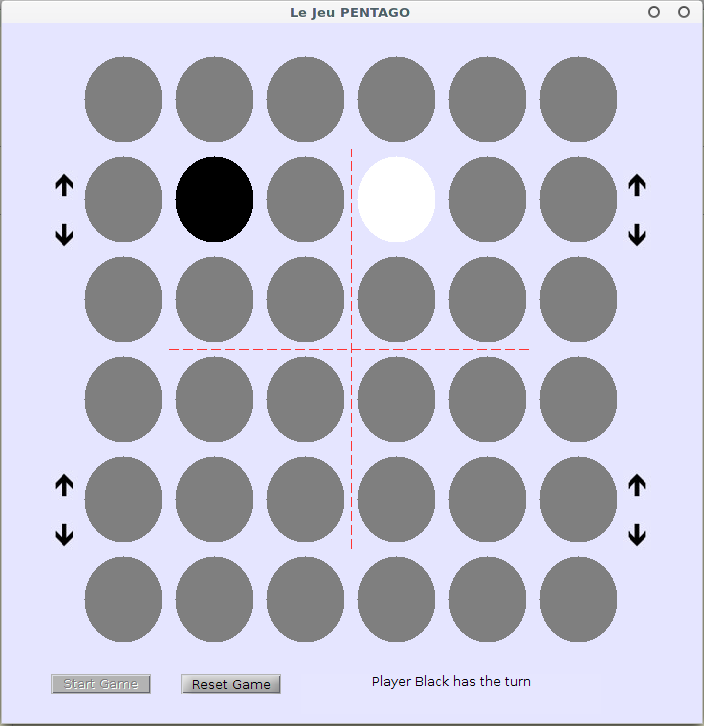
\includegraphics[scale=.35]{images/gui_jeu}
\caption{GUI of our game.}
\label{fig:gui}
\end{figure}

\FloatBarrier

In \textit{MATLAB}, a window is created by the command figure and its
characteristics are defined by some parameters. In our case specifically, the variable plateau
holds a reference for the window and the parameters define some attributes,
such as height, width and screen positions.

\begin{lstlisting}[language=Matlab]
% It creates a new figure which is going to host all the components
plateau = figure ('Visible', 'on', 'Position', [1500, 1000, width, height], ...
    'Name','Le Jeu PENTAGO ','NumberTitle','off', 'Resize', 'off', ...
    'Color', [0.9, 0.9, 1], 'MenuBar', 'none');
\end{lstlisting}

where the variables width and height are started with

\begin{lstlisting}[language=Matlab]
% Board's characteristics
width   = 700;
height  = 700;
\end{lstlisting}

\vspace{10pt}
 
The parameters are detailed below.

\begin{enumerate}    
	\item \textit{Visible} determines whether the window will be visible right next
	it is built.
	\item \textit{Position} is an array containing the coordinates x and y of the
	screen, width and height of the window, respectively.
	\item \textit{Name} is the string that will be displayed in the figure window.
	\item \textit{Number Title} set to ‘off’ means that the string ‘Figure No’ will
	not be displayed in the figure window.
	\item \textit{Resize} set to ‘off’ means that the window cannot be resized.
	\item \textit{Color} sets the background color of the figure.  The array
	contains three values, which determine the color according to the RGB scale. In our case, for instance, 0.9 represents 90% of 255.
\end{enumerate}

Having defined the window, the next step is to determine the axis which the
components are going to be placed in.  For that, we use the command axes, as
shown below.

\vspace{10pt}

\begin{lstlisting}[language=Matlab]
% Board's characteristics
% axes1 represents the total space where we can place our
%       components into
axes1 = axes('Units','Pixels','Position',[50,75,(width - XMargin) , (height - YMargin) ],
    'XLim', [-30 (width - XMargin + 30) ], ...
    'YLim', [0 (height - YMargin) ], 'Color', 'none', 'Visible', 'off');
\end{lstlisting}

\vspace{10pt}

where \textit{XMargin} and \textit{YMargin} specify the empty space between the
margins of the window and the margins of the axes.  They are set to

\vspace{10pt}

\begin{lstlisting}[language=Matlab]
XMargin = 100;
YMargin = 100;
\end{lstlisting}

\vspace{10pt}

In Figure \ref{fig:noeffects}, the role of this component is more clearly
visible. In few words, an axes components plays the role of a ‘painting area’,
which multiple components can be drawn on. The attributes \textit{Color} and
\textit{Visible} specify the color of the axes back planes and the their
visibility, respectively. Setting \textit{Color} to \textit{none} means that the
axes is transparent and the figure color shows through. Setting \textit{Visible}
to \textit{off} prevents axis lines, tick marks, and labels from being
displayed. Attributes \textit{XLim} and \textit{YLim} specifies the minimum and
maximum values of the respective axis.

\begin{figure}[h]
\centering
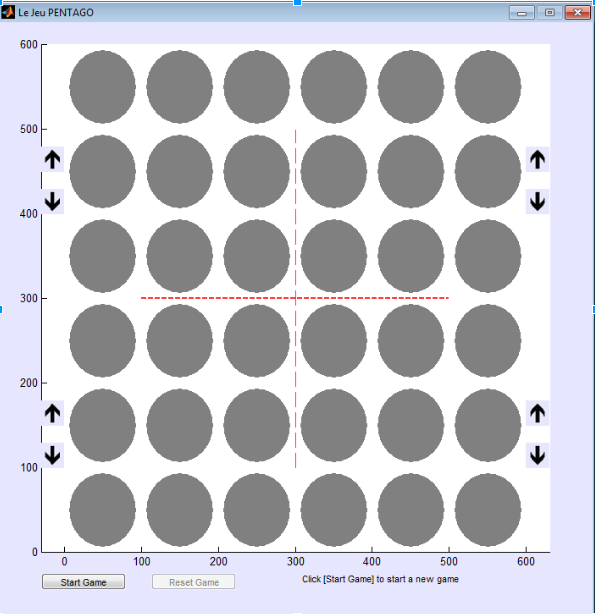
\includegraphics[scale=.43]{images/noeffects}
\caption{\textit{Axis1} with \textit{Color} and \textit{Visible} 
different from \textit{none} and \textit{off}}
\label{fig:noeffects}
\end{figure}

\FloatBarrier

The buttons \textit{Start Game} and \textit{Reset Game} are created by the
command uicontrol, as shown below.

\vspace{10pt}

\begin{lstlisting}[language=Matlab]
% Adds start and reset buttons
buttonStart = uicontrol ('Position', [50 30 100 20], 'String', 'Start Game', ...
    'Callback', @start_pressed);
buttonReset = uicontrol ('Position', [180 30 100 20], 'String', 'Reset Game', ...
    'Enable', 'off', 'Callback', @reset_pressed);
\end{lstlisting}

\vspace{10pt}

The most important parameter is \textit{Callback}. It specifies a function
handler, which will be activated when the button is pressed. In other words,
the function \textit{reset\_pressed} is called right after a mouse click event
over the respective button. 

\vspace{10pt}
 
Despite the fact that each one of the 36 components that compose the board look
like circles, they are obtained by the command rectangle, presented below as well.

\vspace{10pt}

\begin{lstlisting}[language=Matlab]
for l = 1:6
    y = space / 2;
    
    for c = 1:6
        rectangles((6 -(c-1)),l) = rectangle('Curvature', [1.0, 1.0], ...
            'Position', [ x, y , rectWidth-space, rectHeight-space], ...
            'FaceColor', colorRectangle, 'EdgeColor', 'none',...
            'ButtonDownFcn', {@rectangle_pressed,  (6 -(c-1)), l});
        
        y = y + rectHeight;
    end
    
    x = x + rectWidth;
end
\end{lstlisting}

\vspace{10pt}

The circular shape is achieved thanks to the parameter ‘Curvature’, which
specifies the curvature of both rectangle sides. This parameters is composed by
a 2-element array, in which each one of the components can only vary from 0.0
to 1.0. They represent the fraction of width (or height) of the rectangle that
is curved along the top and bottom edges. For example, 0.0 means no curvature
at all and 1.0 creates an ellipse. If both are set to ‘1.0’ and the two sides
are equal, then we will have a circle because an ellipse having all axis with
same length is a circle as well.

\vspace{10pt}

The parameter 'ButtonDownFcn' determines, as the parameter \textit{Callback} in
uicontrol,  the handler of the function that will be called when a circle is
clicked on. The only difference is that, in this case, we will send some
parameters in addition to those that are predefined by MATLAB. l and c
represent the indexes of each button in the matrix. In this way, when an event
is detected, we are able to identify precisely which button has launched it.

\vspace{10pt}

At last, the eight arrows are created by the command image (only two
represented below):

\vspace{10pt}

\begin{lstlisting}[language=Matlab]
% The following lines are responsible for reading the images from the respective files.
% These images correspond to the arrows that make the boards to turn right or left.
rotate_up = imread('arrow_alt_up.jpeg');
rotate_down = imread('arrow_alt_down.jpeg');

% Adds all the eight arrows
textQ1L   = image(-30,450,rotate_down, 'ButtonDownFcn',{@turn_pressed, 1, 'R'});
textQ1R   = image(-30,400,rotate_up, 'ButtonDownFcn',{@turn_pressed, 1, 'L'});
[...]
\end{lstlisting}

\vspace{10pt}

The command imread reads an image from a file and \textit{ButtonDownFcn} has the
same behavior as the cases treated above. It should be noted equally that
turn\_pressed receives as parameters the quadrant (1 in our case) of the
respective arrow and the direction (‘R’ or ‘L’) it represents. ‘-30’ and ‘450’
are the x and y coordinates of the first arrow respectively and ‘-30’ and ‘400’
represent the same for the second one.

\subsection{Game’s Progress}

Once we have programmed all the required components for the GUI, we need to
determine how the program will behave, that is, how each of them will affect
the game’s progress. For that, we need to define some important variables that
are going to represent the game’s state:

\begin{lstlisting}[language=Matlab]
% resets matrix of states.
state_matrix = zeros(6,6);
turn = 'N';
hasTurned = 0;
hasPlayed = 0;
isComputer = 0;
empty_Slots = 36;
\end{lstlisting}

\begin{enumerate}
	\item \textit{turn} specifies which player has the current turn. Initially, the
	turn has no owner, then it is set to ‘N’, standing for Nobody. ‘B’ stands for
	the Black player (by convention, representing the computer) and ‘W’ for White
	(human player).
	\item \textit{state\_matrix} represents the matrix which contains the state of
	every position of the board.
	\item \textit{empty\_Slots} keeps the number of available slots.
	\item \textit{hasTurned} and \textit{hasPlayed} indicate whether the current
	player has turned one of the sub boards and made a move respectively.
	\item \textit{isComputer} indicates if the computer has the current turn. Obs.:
	rigorously we do not need it, because we have already the variable ‘turn’
	controlling the game. However, if, in a not distant future, we desired to
	allow the computer to control the white pieces, we would require this
	variable.
\end{enumerate}

In order to begin a new match, the human player needs to push the button
\textit{Start Button}.  This action will launch an event, that will be processed
by the function \textit{start\_pressed}. At first, the button \textit{Reset
Game} is enabled and \textit{Start Game} disables itself. In other words, it
means that a game can only be reset after the it is started. Next, the function
determines randomly, through the command ‘randi’, whether the human player or
the computer should start playing.  In the first case, we update the state
variables to reflect that decision and wait that player to choose one of the
free slots.

\vspace{10pt}

 When the human player hits one of the circles, another event is created and the
 function rectangle\_pressed assumes the control of the execution. Firstly, it
 checks if that position is really available and if it is not, an error message
 is written in the text space. If the player tries to turn the board before
 playing, an error message will be generated as well. In contradiction with all
 previous statements, the function sets the respective position of
 \textit{state\_matrix}, repaints the board of the figure (function
 \textit{refresh\_board}) and enables the player to turn the board as he wishes
 by setting the variable \textit{hasPlayed} to 1.
 

\vspace{10pt}

The human player is allowed then to press one of the eight arrows along the
board. Doing so, he produces an event, which is processed by the function
\textit{turn\_pressed}.  This routine verifies if the player can do this and, in
the positive case, the matrix state and the board are updated (functions
\textit{rotate\_quadrant} and \textit{refresh\_board} respectively) and
\textit{hasTurned} is set to 1. Finally, it calls another function,
\textit{verify\_turn\_changing}, which is responsible to verify some conditions,
such as whether the game has finished or there is not available slots anymore,
and to change the turn if nobody has won yet (function \textit{change\_turn}). 
In this last case, the function calls then one of the routines which implement
an algorithm of artificial intelligence (see next sections), which returns the
move, quadrant and sense of rotation that the computer has chosen to make. The
last step is to update the state variables and repaint the board.

\vspace{10pt}

If the computer has been selected to start the game, then this last  process is
done before any move of the human player.

\vspace{10pt}

The  human player can press the \textit{Reset button} at any time. When this
happens, the function \textit{reset\_pressed} is called. This routines restores all state
variables and board to their initial conditions, enables the \textit{Start
button} and disables itself. In the way as before, a game can only be started if
it has been reset.

\subsection{Evaluating a board}

All code used in this section can be found in file \textbf{evaluate\_board.m}.

\vspace{10pt}

The best algorithm ever created would not be enough if we did not have a way of
evaluating a board efficiently. For that reason, we developed a method capable
of detecting the presence of lines, columns and diagonals contained in the
matrix  of states. This function is named \textit{evaluate\_board} and receives
as parameters the state matrix and the player for whom the board will be
evaluated.

\vspace{10pt}

This routine uses essentially six variables to count the total score of a
board:
 
 \vspace{10pt}

\begin{lstlisting}[language=Matlab]
hasBeenDetected = zeros(6,6);
playerScores = zeros (4,1);
opponentScores = zeros (4,1);
scores = [playerScores  opponentScores];
foundUltraCondition = 0;
value = 0;
\end{lstlisting}

\begin{enumerate}
  	\item \textit{value} is the result that will be given to that board.
	\item Each element of \textit{hasBeenDetected} is an integer whose
	representation in binary determines if that element has already been detected
	taking place in at least one line/column or diagonal. 0001 means that it takes
	place in a COLUMN, 0010 in a LINE, 0100 in a DIAGONAL to the right and 1000 in
	a DIAGONAL to the left. For example, if hasBeenDetected(i, j) is 0011, it
	means that position forms a LINE and a COLUMN at the same time.
	\item \textit{playerScores} is an array that stores the scores of all
	combination the player’s got so far in each one of the possible configurations (COLUMN, LINE and DIAGONALS). For example, if the player has a 3-element line, then playerScores(2,1) receives the score for that combination.
	\item \textit{opponentScores} is the same but for the opponent.
	\item \textit{scores} is the matrix containing both playerScores and
	opponentScores.
	\item The column concerning player is the first one and the column concerning
	the opponent is the last one. Its use is going to be discussed in the following
	lines.
	\item \textit{foundUltraCondition} is true if we detect a line, column or
	diagonal completely filled with 5 pieces.
\end{enumerate} 

Once that the variables were initialized, the routine verifies whether each
filled position (x,y) of the matrix of states forms a possible combination.
In order to do that, we introduce another index, \textit{offset\_index}, which
starts at 4 and is decremented by 1 every iteration. This process stops when
\textit{offset\_index} reaches 0.  It is used to retrieve a line, column or
diagonal of length equivalent to 1 + \textit{offset\_index}, as it is shown
below.

\vspace{10pt}

\begin{lstlisting}[language=Matlab]
t = state_matrix (x:(x+offset_index) , y);
\end{lstlisting}

\vspace{10pt}

It is evident that we need to verify that (x+offset\_index) respects the
dimension of state\_matrix before executing the previous command.

\vspace{10pt}

Next, we need to verify if all elements of t are the same. For that, we execute
the following command, provided by MATLAB:

\vspace{10pt}

\begin{lstlisting}[language=Matlab]
if all(t == t(1)) [...]
\end{lstlisting}

\vspace{10pt}

If that condition is true, then we refer once more to \textit{offset\_index}. If
it is equal to 4 and all elements are the same, then we do not need to verify the
other elements, because this situation is equivalent to the maximum or minimum
score, depending on the value of \textit{state\_matrix(x,y)} (if it is equal to
\textit{player}, it is maximum, minimum otherwise). We set then
foundUltraCondition to 1, which is going to stop all loops (those ones that iterate x and y and that one which
iterates \textit{offset\_index}).

\vspace{10pt}

The number of filled positions and the score that the combination generates are
then stored in the matrix scores, introduced before, the respectives columns
depending on the player. The code below implements the solution.

\vspace{10pt}

\begin{lstlisting}[language=Matlab]
scores(1, index_player) = scores(1, index_player) + 10^(3*(offset_index+1));
\end{lstlisting}

\vspace{10pt}

\textit{index\_player} determines the columns that are accessed: if the current
position we are verifying corresponds to the player, then \textit{index\_player}
is 1 and the first column is modified. If not, then \textit{index\_player} is set to 2
and the second column of scores is accessed. It should be noted as well that
all the scores are added up. So, the result of a board is as big as the number
of combinations. In this way, the computer always prefers to increase the number
of combinations (refer to section \textbf{Searching the best move}).

\vspace{10pt}

The last thing to do is to update hasBeenDetected with the positions of each
element composing the combination. That prevents that the same element is
counted two or more times for the same combination. For example, let’s consider
that the positions (i,j), (i, j+1) and (i, j+2) are filled and
compose therefore a three-element line. (i, j) is iterated before the others
and the score is given according to the size. If hasBeenDetected had not been update,
then the program would counter (i, j+1) and (i, j+2) as another
two-element line, what is evidently false because it has been already counted. For a line,
each position of hasBeenDetected with same coordinates than the line present in
\textit{state\_matrix} is added up with 2 (0010 in binary).

\vspace{10pt}

\begin{lstlisting}[language=Matlab]
% fills hasBeenDetected with 0010 in the
% respective LINE
hasBeenDetected (x , y:(y + offset_index)) =  ... 
	hasBeenDetected (x , y:(y + offset_index)) + 2;
\end{lstlisting}

\vspace{10pt}

Additionally, if there is only one element that are not equal in the combination
(for example, a column composed by 4 black pieces and only one white piece),
then we attribute an intermediate score between the points that a complete
combination would receive and the points that 4-element combination would have.
This means that the computer would rather save its own skin before forming a
4-element configuration (refer to section \textbf{Searching the best move}).

\vspace{10pt}

The last thing the function does is summing up everything up to obtain the final
result of the current board:

\vspace{10pt}

\begin{lstlisting}[language=Matlab]
value =  value + sum(scores(:, 1) - scores(:, 2));
\end{lstlisting}

\subsection{Searching for the best move}

\subsubsection{The choice of the algorithm}


It may be trivial that, with infinite time available, one might easily solve
most games just by exploring the full game-tree. As it is not the case in real
world, one has to implement search algorithms that reduces the complexity of
the problem and run on an acceptable amount of time.

\vspace{10pt}

There are many available methods for searching the best move in two players
zero-sum games with perfect information, being the most commons: Alpha-Beta
Search (and variants), Proof-Number Search (and variants), Threat-space Search
and Retrograde search (<<On solving Pentago, 2015>>).

\vspace{10pt}

For this project, we have chose to implement the Alpha-Beta Search, as it is
the most common algorithm for solving Pentago. Moreover, this algorithm
presents great many interesting variants, that are commonly employed on AIs,
and therefore well comprehending him is a good asset to well understand the
more elaborated solutions available.

\vspace{10pt}

As for the complexity of this approach, (Russell, Stuart J., 2003) explains
that with an (average or constant) branching factor of b, and a search depth of
d plies, the maximum number of leaf node positions evaluated (when the move
ordering is pessimal) is \( \mathcal{O}( b*b*...*b ) = \mathcal{O}( bd ) \) –
the same as a simple minimax search. If the move ordering for the search is
optimal (meaning the best moves are always searched first), the number of leaf
node positions evaluated is about \(\mathcal{O}(b*1*b*1*...*b)\) for odd depth
and \(\mathcal{O}( b*1*b*1*...*1 ) \) for even depth, or \(\mathcal{O}(
\frac{bd}{2} ) = \mathcal{O}( \sqrt { bd }  ) \). In the latter case, where the
ply of a search is even, the effective branching factor is reduced to its
square root, or, equivalently, the search can go twice as deep with the same
amount of computation. Meanwhile, (McCarthy, 2006) poses that when nodes are
ordered at random, the average number of nodes evaluated is roughly \(\mathcal{O}(
b(\left( \frac{3*d}{4} \right)) )\).

\vspace{10pt}

The Alpha-Beta Search or the Alpha-Beta pruning is based on the minimax
algorithm but presents a new feature: it is capable of <<pruning>>, skipping an
area - subtree - of the search that is not capable of affecting the result of
the search. The (Standford University, 2015) presents the following general
description:

\begin{enumerate}
  	\item Consider a node n somewhere in the tree, such that one can move to that
  	node.
	\item  If there is a better choice m either at the parent of the node n or at
	any choice point further up, n will never be reached.
	\item Once we have enough information about n to reach this conclusion, we can
	prune it.
\end{enumerate}

Alpha-Beta pruning gets its name from the following parameters:

\vspace{10pt}

\(\alpha \) = the value of the best choice we have found so far at any choice
point along the path for MAX. 

\(\beta\) = the value of the best choice we have found so far at any choice
point along the path for MIN

\vspace{10pt}
[...] Alpha-Beta search updates the values of \(\alpha \) and \(\beta\) as it
goes along and prunes the remaining branches at a node as soon as the value of
the current node is known to be worse than the current values of \(\alpha\) and
\(\beta\).

\vspace{10pt}
It is possible to synthesize this behavior with pseudo-code - translation to English from the one available on (Élagage alpha-beta, 2015) in French - :

\vspace{10pt}

\begin{lstlisting}[language=Java]
function ALPHABETA(P, alpha, beta) /* alpha always smaller than beta*/
   if P is leaf then
       return the value of P
   ifelse
       if P is Min node then
           Val = infinite
           for each children Pi of P do
               Val = Min(Val, ALPHABETA(Pi, alpha, beta))                
               if alpha >= Val then  /* alpha cutoff*/
                   return Val
               endif    
               beta = Min(beta, Val)
           endfor            
       ifelse
           Val = -infinite
           for each children Pi of P do
               Val = Max(Val, ALPHABETA(Pi, alpha, beta))                
               if Val >= beta then /*beta cutoff */
                   return Val
               endif   
               alpha = Max(alpha, Val)
           endfor
       endif
   return Val
   endif
end
\end{lstlisting}

\vspace{10pt}

An execution  of the alpha-beta pruning is illustrated below (Chalmers -
GÖTEBORGS UNIVERSITET, 2015):

\begin{figure}[h]
\centering
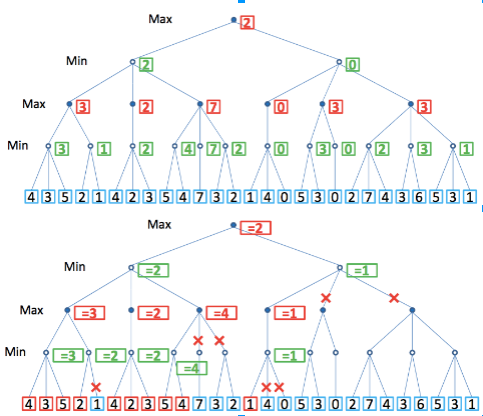
\includegraphics[scale=.75]{images/minmax}
\caption{Illustration of an alpha-beta pruning run.}
\label{fig:minmax}
\end{figure}

\FloatBarrier

\subsubsection{Coding}

All code used in this section can be found in the file
\textbf{alpha\_beta\_search.m}.

\vspace{10pt}

First, we establish what the function will return: the evaluation of the
board(\textit{eval\_value}), the place([line column]) where the next piece will
be played(move), the quadrant where the rotation is applied after the piece be
placed (quadrant) and the direction of the rotation (direction). This may be
encapsulated in an array using Matlab's succinct syntax.

\vspace{10pt}

\begin{lstlisting}[language=Matlab]
function [eval_value move quadrant direction] = alpha_beta_search (state_matrix, 
				emptySlots, depth, alpha, beta, isMaximizing, player)
\end{lstlisting}

\vspace{10pt}

Second, we establish the base case of our recursive call, triggered by reaching
the final depth of exploration. This is indicated by the variable depth when it
reaches 0.

\vspace{10pt}

\begin{lstlisting}[language=Matlab]
if depth == 0 || emptySlots == 0
    
    [eval_value] = evaluate_board(state_matrix, player);
    move = [];
    quadrant = 0;
    direction = 0;
[...]
\end{lstlisting}

\vspace{10pt}

Finally, we do the actions required for the alpha beta pruning when it does not
find itself in the base case. If that is the case, we will firstly initialise
the variables used in the alpha beta search (alpha, beta) and our supplemental
variable that allows us to do the pruning (mustStop). The supplemental variable
will do so by breaking the while loops that are used to explore our tree, since
\textit{mustStop = 0} will imply skipping further branches.

\vspace{10pt}

\begin{lstlisting}[language=Matlab]
[...]
else   
    dir = ['L' 'R'];
    mustStop = 0;
    
    if (isMaximizing == 1)
        eval_ = -inf;
    else
        eval_ = +inf;
    end
\end{lstlisting}

\vspace{10pt}

Then, we will proceed to explore our <<tree>> . In fact, instead of using a tree
structure itself to explore the possible outcomes of the plays and implement
the prunings, we will rather use a cascade of while loops that will break if we
arrive to a natural limit of our tree - for instance, we will not explore the
plays that may involve playing a piece in the 7th line of our board, since our
board does not have a 7th line - or if the further branches are pruned by the
alphabeta algorithm  - that is signaled by the mustStop supplemental variable
described above -.

\vspace{10pt}

The process begins by setting a piece of the color of the player (variable
<<player>>) which the turn is ongoing while the \textit{alpha\_beta\_search}
function is being used if we are in a maximizing phase or by placing a piece of
the opposite colour if we are in a minimizing phase. After that, we will rotate
one of the quadrants to one of the possible directions.

\vspace{10pt}

One might notice that the combination of line, column, piece played, quadrant
of rotation and rotation direction plays a role analogue to a node in the tree
structure.

\vspace{10pt}

\begin{lstlisting}[language=Matlab]
[...]
l = 1;
while (l <= 6) && (mustStop == 0)
    
    c = 1;
    while (c <= 6) && (mustStop == 0)
        
        if state_matrix (l,c) == 0

            quad_index = 1;
            while (quad_index <=4) && (mustStop == 0)
                
                dir_index = 1;
                while (dir_index <= 2) && (mustStop == 0)
                    
                    if isMaximizing == 1
                        state_matrix (l,c) = player;
                    else
                        
                        if player == 'B'
                            state_matrix (l,c) = 'W';
                        else
                            state_matrix (l,c) = 'B';
                        end
                        
                    end
                    
                    state_matrix = rotate_quadrant (state_matrix, quad_index,
                    	 dir (dir_index) );
                    [...]
\end{lstlisting}

\vspace{10pt}

Afterwards, we will apply the \textit{verify\_victory} function over the board
that we are exploring to determine the state of the game, which may assume the values:
white player is victorious(‘W’), black player is victorious(‘B’), we have a
draw (‘D’) or the game is not yet over ( 0 ). The \textit{verify\_victory}
function may be found in the file \textbf{verify\_victory.m}.

\vspace{10pt}

Knowing the state of the game, we may shortcut some decisions: if a player
finds that by doing a certain move he will imply that the other player right
after counter attack with a winning play, he will avoid the play that would led
to his defeat by any means. He will not do it unless there are no possible play
that will not lead to a defeat. That line of thinking is implemented by giving
that board an evaluation so low that it can be outmatched by any non losing
board.

\vspace{10pt}

In a similar way, if he finds a play that leads to his victory, he will no
further explore the possible plays that may be done in that board: the play
that he will do is already clear, we can not get better than a clear win. That
is implemented by giving that board an evaluation so high it can not be
outmatched by a non winning board.

\vspace{10pt}

Moreover, we will update the alpha and beta parameters following the rules
previously explained that characterise the alpha-beta pruning. Furthermore,
\textit{mustStop} value will be update as well, in order to enable the pruning
when it may be done.

\vspace{10pt}

\begin{lstlisting}[language=Matlab]
[...]
state_game_ = verify_victory(state_matrix);
                        
if isMaximizing == 1 && (state_game_ ~= 0) && (state_game_ ~= 'D')
    
    if state_game_ == player
        eval_MIN = +10^20;
        mustStop = 1;
    else
        [eval_MIN move_MIN quadrant_MIN direction_MIN] = ...
            alpha_beta_search(state_matrix, emptySlots - 1, depth - 1, alpha, beta, 0, player);                        
    end
    
    if eval_ < eval_MIN
        
        eval_ = eval_MIN;
        eval_value = eval_;
        move = [l c];
        quadrant = quad_index;
        direction = dir (dir_index);
        
    end
    
    if eval_ >= beta
        mustStop = 1;
    end
    
    alpha = max(alpha, eval_);
    
    
elseif isMaximizing == 0
    
    if (state_game_ ~= player) && (state_game_ ~= 0) && (state_game_ ~= 'D')
        eval_MAX = -10^20;
        mustStop = 1;
    else
        [eval_MAX move_MAX quadrant_MAX direction_MAX] = ...
            alpha_beta_search(state_matrix, emptySlots - 1, depth - 1, alpha, beta, 1, player);
    end
    
    if eval_ > eval_MAX
        
        eval_ = eval_MAX;
        eval_value = eval_;
        move = [l c];
        quadrant = quad_index;
        direction = dir (dir_index);
        
    end
    
    if alpha >= eval_
        mustStop = 1;
    end
    
    beta  = min(beta, eval_);
end
[...]
\end{lstlisting}

\vspace{10pt}

Lastly, we will restore the state of our board(\textit{state\_matrix}) to how it
was before doing the play that we are analysing, hence enabling the board to be
reused by the following play that we will analyse. This is done by doing the
reverse of all modifications that we have applied since we run the alpha beta
search on the board.

In addition to that, we will update our loops parameters and restart our loop.

\vspace{10pt}

\begin{lstlisting}[language=Matlab]
	if dir (dir_index) == 'L'
		state_matrix = rotate_quadrant(state_matrix, quad_index, 'R');
	else
		state_matrix = rotate_quadrant(state_matrix, quad_index, 'L');
	end

	state_matrix (l,c) = 0;
	dir_index = dir_index + 1;
end
quad_index = quad_index + 1;
end
[...]
\end{lstlisting}

\subsubsection{Battle of AIs - A statistical point of view}
                        

In order to determine whether our algorithm is effectively good in terms of
strategy and time, we wrote two other programs that basically simulate a match
between two artificial intelligences - the one did and the other done by our
advisor. The first program,
\textbf{pentago\_plateau\_graphical\_battle\_of\_IAs.m}, offers a graphical
interface, which enables the user to follow every move taken by the algorithms.
This function was adapted from the procedure explained in the previous
sections, thus its characteristics are almost the same. The second one,
\textbf{pentago\_plateau\_simple\_battle\_of\_IAs.m}, does not provide a
graphical interface but is able of simulating any number of matches in a row.
Consequently, this function is faster and suits better a statistical study.

\vspace{10pt}

We decided to focus our analysis on two different parameters: the time which is
required for each algorithm to decide its next move and the number of victories
of each AI. In order to do that in the fairest way and considering that PENTAGO
is a first-player game, each AI has the first move in exactly half of the 500
simulated matches, that is 250 matches. The code of this analysis is present in
file \textbf{process\_information.m}.


\vspace{10pt}

Concerning the number of victories, the player White, which represents our AI,
won a total of 193 out of 500, while the player Black, our advisor’s AI,
succeeded in 223 matches. The rest of them, 84 matches, represents evidently
the draws. The figure \ref{fig:hist} summarizes these results. As we can see,
the player White won 90 of its victories when the other player started playing and 103
otherwise. With respect to player Black, it won the most of its victories, 116,
when it had the first move. The rest, 107 matches, were evidently won when
player White had the preference. As for the draws, 44 were observed when player
Black started and 40, when the other player had the first move.

\begin{wrapfigure}{r}{0.5\textwidth}
  \vspace{-40pt}
  \begin{center}
    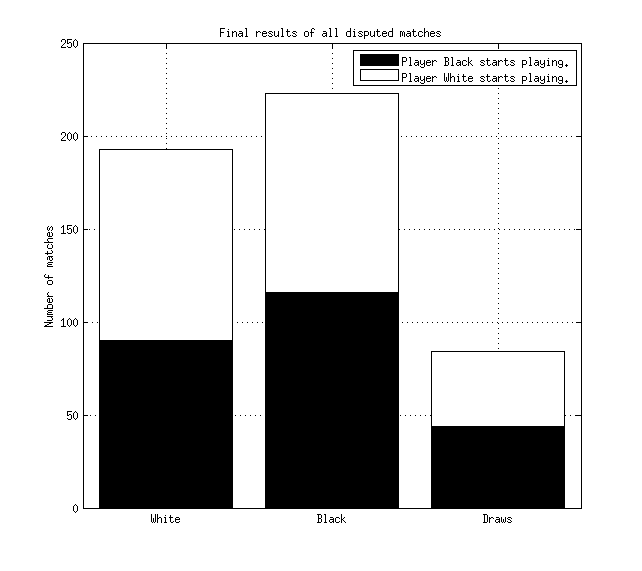
\includegraphics[width=0.50\textwidth]{images/victories_count}
  \end{center}
  \vspace{-20pt}
  \caption{Number of victories of each player.}
  \vspace{-30pt}
  \label{fig:hist}
\end{wrapfigure} 
\vspace{10pt}

Based on the previous results, we can observe that:

\begin{itemize}
  \item Our advisor’s algorithm presents a slightly better strategy than ours.
  Its chance of winning can be estimated at 44.6\%, whereas ours can be
  estimated at 38.6\%. Finally, a draw has the probability of 16.8\% of
  occurring.
  \item  The fact of starting the game has really an effect in the final result.
  Player White has a probability of 41.2\% given that it started. The
  probability for player Black is slightly bigger: 46.4\% of chance given that
  it’s him that starts the match.
\end{itemize}

In relation to the time required to the calculations, the figures
\ref{fig:time_white} and \ref{fig:time_black} show the results that were
obtained for the 500 matches. We must consider that we used our own personal
computers, that are not naturally designed to run simulations. Additionally,
their resources were not dedicated exclusively for this experiment (‘Midterm
exams are coming!’).


\begin{figure}[h]
        \centering
        \begin{subfigure}[b]{0.5\textwidth}
                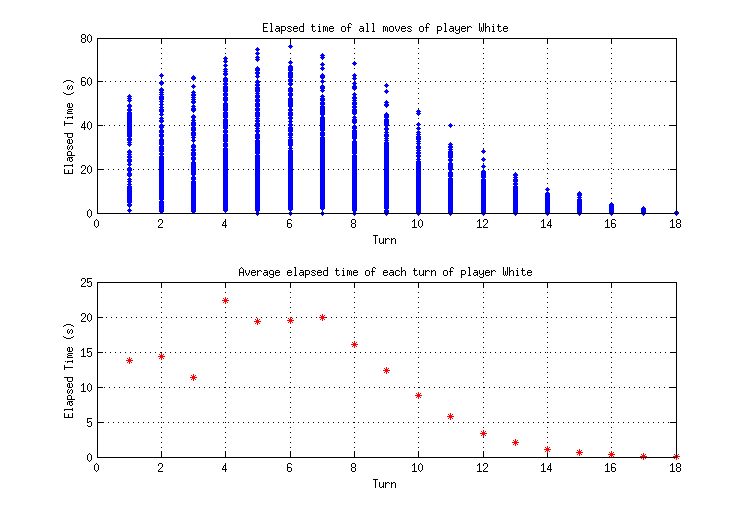
\includegraphics[width=\textwidth]{images/PENTAGOtimes}
                \caption{Required time to Player White take a move.}
                \label{fig:time_white}
        \end{subfigure}%
        ~ %add desired spacing between images, e. g. ~, \quad, \qquad, \hfill etc.
          %(or a blank line to force the subfigure onto a new line)
        \begin{subfigure}[b]{0.5\textwidth}
                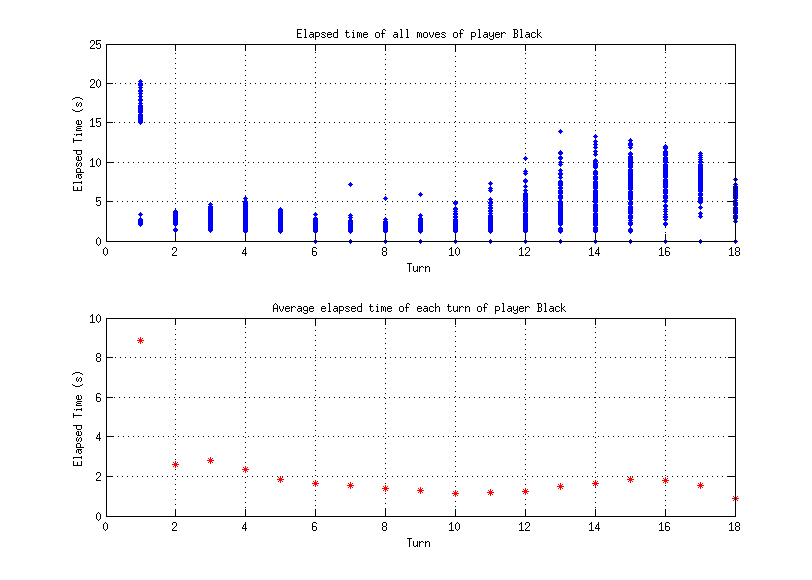
\includegraphics[width=\textwidth]{images/LBtimes}
                \caption{Required time to Player Black take a move.}
                \label{fig:time_black}
        \end{subfigure}

\end{figure}

\FloatBarrier

The upper plots of each figure, in blue, are simple representations of the
times which are saved right after each move was decided. In other words, each
blue point stands for the time required to calculate every move. The plots
containing red symbols show, for each turn, the average time required to decide
that move. We observe then:

\begin{itemize}
	\item Player White takes, in average, 9.5 seconds to decide. Player Black takes
	2.05 seconds. The difference between these two times is explained by how which
	algorithm decides the move and evaluates a board. As explained before, our
	algorithm needs to verify each position of the matrix at least twice: once to
	evaluate if that position belongs to a row, column or diagonal, and another to
	conclude if that move is profitable.
	\item Player White’s initial moves take longer times, meanwhile the delay of
	the latest moves decreases. That’s already expected by the same reason we had
	before: at the beginning of the  match, there are more positions to be
	verified, contrarily to the end, in which few available positions remain.
	\item Player Black's moves takes roughly constant time, around 2 seconds, to
	be decided. The only move that does not follow that property is the first one.

\end{itemize}

\newpage